\documentclass{article}

% set font encoding for PDFLaTeX, XeLaTeX, or LuaTeX
\usepackage{ifxetex,ifluatex}
\if\ifxetex T\else\ifluatex T\else F\fi\fi T%
  \usepackage{fontspec}
\else
  \usepackage[T1]{fontenc}
  \usepackage[utf8]{inputenc}
  \usepackage{lmodern}
\fi
\usepackage[landscape]{geometry}% http://ctan.org/pkg/geometry
\usepackage{array}% http://ctan.org/pkg/array
\usepackage{hyperref}
\usepackage{tikz}
\usepackage{xcolor}
\usepackage{fullpage}
\usepackage{xifthen}
\usepackage{setspace}
\usepackage{xstring}
\usepackage{comment}
\usepackage{listings}
\usetikzlibrary{circuits.logic.US,circuits.logic.IEC,fit}
\newcommand\addvmargin[1]{
  \node[fit=(current bounding box),inner ysep=#1,inner xsep=0]{};
}

\def\arraystretch{1.5}%  1 is the default, change whatever you need

%% Colors
\definecolor{cbeige}{HTML}{FAEBD7}
\definecolor{cpink}{HTML}{FFC0CB}
\definecolor{cblack}{HTML}{010101}
\definecolor{corange}{HTML}{D2691E}
\definecolor{cred}{HTML}{FF0921}
\definecolor{cpurple}{HTML}{9683EC}
\definecolor{cyellow}{HTML}{FEF86C}
\definecolor{clightgreen}{HTML}{BEF574}
\definecolor{cdarkgreen}{HTML}{82C46C}
\definecolor{cskyblue}{HTML}{E0FFFF}
\definecolor{cgrey}{HTML}{8A8A8A}

% Couleurs utilisées dans l'exemple du disque
\definecolor{cmarron}{HTML}{AE8964}
\definecolor{cfuschia}{HTML}{ff1493}
\definecolor{climegreen}{HTML}{00ff00}
\definecolor{ccrememarron}{HTML}{cd853f}
\definecolor{clavender}{HTML}{da70d6}
\definecolor{clightgrey}{HTML}{f0f8ff}
\definecolor{cbordeau}{HTML}{a52a2a}
\definecolor{csuperblue}{HTML}{7fffd4}
\definecolor{cbrun}{HTML}{d2691e}
\definecolor{cocean}{HTML}{00ced1}
\definecolor{ckaki}{HTML}{556b2f}
\definecolor{cpika}{HTML}{ffd700}
\definecolor{clouche}{HTML}{696969}




%% Macros
% 
\newcommand{\coloritem}[2]{\IfSubStr{|cbeige|cpink|cmarron|cblack|corange|cred|cpurple|cyellow|clightgreen|cdarkgreen|cskyblue|cgrey|cfuschia|climegreen|ccrememarron|clavender|clightgrey|cbordeau|csuperblue|cbrun|cocean|ckaki|cpika|clouche|}{#1}
{\draw[black,fill=#1] (#2) circle (.25);}
{\draw (#2) node (.25) {#1};\draw[black] (#2) circle (.25);}}

% Circles
\newcommand\ccircle[1]{
\begin{tikzpicture}
  \draw[black,fill=#1] (0,0) circle (.25);
\end{tikzpicture}
}

% Tasks
\newcommand\twotaskscircles[2]{
\begin{tikzpicture}

  \coloritem{#1}{0,0}
  \draw[] (.8,0) node[]{$+$};
  \coloritem{#2}{1.6,0}
  \draw[] (2.4,0) node[]{$=$};

\end{tikzpicture}
}




\newcommand\threetaskscircles[3]{
\begin{tikzpicture}

  \coloritem{#1}{0,0}
  \draw[] (.8,0) node[]{$+$};
  \coloritem{#2}{1.6,0}
  \draw[] (2.4,0) node[]{$+$};
  \coloritem{#3}{3.2,0}
  \draw[] (4,0) node[]{$=$};
  
  \draw[] (4.5,0) to (4.5,3)  ;
  

\end{tikzpicture}
}




\newcommand\fourtaskscircles[4]{
\begin{tikzpicture}

  \coloritem{#1}{0,0}
  \draw[] (.8,0) node[]{$+$};
  \coloritem{#2}{1.6,0}
  \draw[] (2.4,0) node[]{$+$};
  \coloritem{#3}{3.2,0}
  \draw[] (4,0) node[]{$+$};
  \coloritem{#4}{4.8,0}
  \draw[] (5.6,0) node[]{$=$};

\end{tikzpicture}
}

\newcommand\taskname[1]{
\begin{tikzpicture}
\draw node[above,minimum size=2ex]{\texttt{#1}};
\end{tikzpicture}
}

\newcommand\twotask[3]{
\scalebox{1.4}{
\parbox{5cm}{
\setlength{\extrarowheight}{5pt}%
\begin{tabular}{|c|c|c|}
\hline
 \taskname{#1} & \twotaskscircles{#2}{#3} & \ccircle{white}\\
\hline
\end{tabular} \vspace{1ex}
}
}}

\begin{comment}


\newcommand\threetask[4]{
\scalebox{1.4}{
\parbox{5cm}{
\setlength{\extrarowheight}{5pt}%
\begin{tabular}{|c|c|c|}
\hline
 \taskname{#1} & \threetaskscircles{#2}{#3}{#4} & \ccircle{white}\\
\hline
\end{tabular} 
}
}}

\end{comment}









\newcommand\fourtask[5]{
\scalebox{1.4}{
\parbox{5cm}{
%


 
 \begin{tikzpicture}
 %\draw node[above,minimum size=2ex]{\texttt{#1}};
 \draw (-1.8,0)  rectangle (10.5,0.8);
 \draw (-0.5,0.1)  rectangle (4,0.7);
 \draw (2.75,0.05)  rectangle (7.5,0.75);
 
 \draw [-] (6.5,0.05) to (6.5,0.75);
 
 \draw [-] (9.5,0) to (9.5,0.8);
 
 
 \draw[] (8.0,0.4) node[]{$+$};
 \coloritem{#5}{8.7,0.4}
 
 \draw[black,fill=white] (10,0.4) circle (.25);
 
 \coloritem{#2}{0,0.4}
  \draw[] (.8,0.4) node[]{$+$};
  \coloritem{#3}{1.6,0.4}
  \draw[] (2.4,0.4) node[]{$=$};
  
  \draw[] (2.75,0.1) to (2.75,0.7) ;
  
  \draw[black,fill=white] (3.2,0.4) circle (.25);
  
  \draw[] (4.4,0.4) node[]{$+$};
  \coloritem{#4}{5.2,0.4}
  \draw[] (6,0.4) node[]{$=$};
  \draw[black,fill=white] (7,0.4) circle (.25);
  
  \draw [-] (-0.9,0) to (-0.9,0.8);
  
  
  
  \draw (-1.3,.45) node {#1};
  
  
  
  
  
   \, \, \, \,\, \,\, \,\, \,\, \,\, \,\, \,\, \,\, \,\, \,\, \,
 %\draw[black,fill=#2] (0,0.4) circle (.25);
 
 


\end{tikzpicture}  
}}\vspace{2mm}}








\newcommand\threetask[4]{
\scalebox{1.4}{
\parbox{5cm}{
%


 
 \begin{tikzpicture}
 %\draw node[above,minimum size=2ex]{\texttt{#1}};
 \draw (-1.8,0)  rectangle (7.5,0.8);
 \draw (-0.5,0.1)  rectangle (4,0.7);
 
 
 
 \coloritem{#2}{0,0.4}
  \draw[] (.8,0.4) node[]{$+$};
  \coloritem{#3}{1.6,0.4}
  \draw[] (2.4,0.4) node[]{$=$};
  
  \draw[] (2.75,0.1) to (2.75,0.7) ;
  
  \draw[black,fill=white] (3.2,0.4) circle (.25);
  
  \draw[] (4.4,0.4) node[]{$+$};
  \coloritem{#4}{5.2,0.4}
  \draw[] (6,0.4) node[]{$=$};
  \draw[black,fill=white] (7,0.4) circle (.25);
  
  \draw [-] (-0.9,0) to (-0.9,0.8);
  
  \draw [-] (6.5,0) to (6.5,0.8);
  
  \draw (-1.3,.45) node {#1};
  
  
  
  
  
   \, \, \, \,\, \,\, \,\, \,\, \,\, \,\, \,\, \,\, \,\, \,\, \,
 %\draw[black,fill=#2] (0,0.4) circle (.25);
 
 \vspace{1ex}
 

\end{tikzpicture} 
}
} \vspace{2mm}
}




%\title{Tasks}
%\author{Me & Me}

% Enable SageTeX to run SageMath code right inside this LaTeX file.
% http://doc.sagemath.org/html/en/tutorial/sagetex.html
% \usepackage{sagetex}

% Enable PythonTeX to run Python – https://ctan.org/pkg/pythontex
% \usepackage{pythontex}

\begin{document}

\begin{center}
    {\Large\textbf{Problème 1 - Tâches}}
    \vspace{10mm}
\end{center}

\begin{minipage}[b]{0.27\textwidth}  

    \centering  

        \twotask{A}{clouche}{cbrun}
        
        \twotask{B}{ckaki}{cocean}
        
        \twotask{L}{cbordeau}{D}
        
        \twotask{D}{ckaki}{cpika}
    
        \twotask{E}{A}{B}
        
        \threetask{K}{ccrememarron}{climegreen}{cfuschia} 
        
        \fourtask{C}{cmarron}{ccrememarron}{climegreen}{cfuschia} 
        
\end{minipage}
\hfill
\begin{minipage}[b]{0.27\textwidth}
    \centering

        \twotask{F}{B}{C}
        
        \twotask{G}{C}{D}
        
       \twotask{H}{E}{F}
      
        \twotask{I}{F}{G}
        
        \twotask{J}{H}{I}
        
        \vspace{+27.8mm}

\end{minipage}
\hfill
\begin{minipage}[b]{0.27\textwidth}
    \centering
        
        \twotask{M}{cpika}{F}
        
        \twotask{N}{J}{K}
        
        \twotask{O}{N}{L}
        
        \twotask{P}{O}{M}
        
        \vspace{+27.8mm}
        
\end{minipage}


\newpage

\begin{center}
    {\Large\textbf{Problème 1 - Graphe de dépendances}}
\end{center}

\begin{figure}[ht]
    \centering
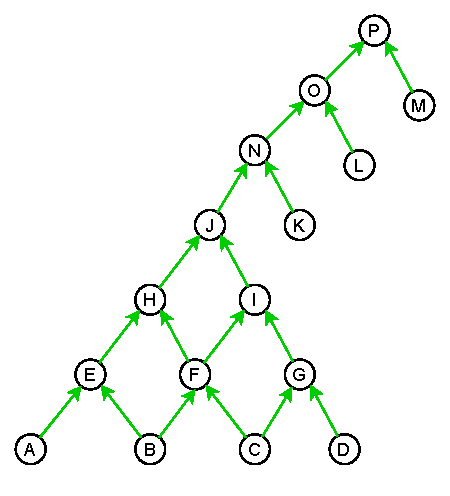
\includegraphics[scale = 1.3]{assets/graph.pdf}
\caption{Graphe de dépendances}
\label{fig:graphe}
\end{figure}

Dans le graphe de la Figure~\ref{fig:graphe}, les noeuds représentent les noms des tâches, et les arêtes représentent les dépendances entre les tâches. Plus précisément, une arête relie la tâche $A$ à la tâche $E$ si on a besoin de la tâche $A$ pour réaliser $E$. Ce graphe est plus communément appelé graphe de dépendances. Déterminer le chemin critique (i.e. le chemin le plus long) dans ce type de graphe, permet de donner un ordre des tâches à réaliser. Une idée intéressante pour débuter est donc de commencer par réaliser les tâches du chemin critique (voir méthode PERT).


\newpage

\begin{center}
    {\Large\textbf{Créer une activité}}
\end{center}

\begin{minipage}[b]{0.30\textwidth}  
        Des tâches peuvent être créées facilement en ajoutent une page à ce fichier LaTeX. Une tâche de taille 2, 3 ou 4 peut être créée à l'aide des macros \lstinline|\twotask|, \lstinline|\threetask| and \lstinline|\fourtask|. Le premier argument dénote le nom de la tâche, et devrait être une lettre
\end{minipage}
\hfill
\begin{minipage}[b]{0.30\textwidth}
    simple. Les arguments qui viennent ensuite donnent les couleurs que l'on verra sur les tâches. Si la valeur de l'argument est égale à une couleur telle que définie dans le fichier \lstinline|macro.tex|, alors l'argument sera interprété comme tel. Sinon, la valeur de l'argument
\end{minipage}
\hfill
\begin{minipage}[b]{0.30\textwidth}
        sera écrite telle quelle. Pour modifier les couleurs, il faut modifier le fichier \lstinline|macro.tex|. Pour ajouter des couleurs, il suffit de rajouter la commande associée dans \lstinline|macro.tex|, puis d'ajouter le nouveau nom dans la liste définie dans la commande \lstinline|\coloritem|.
\end{minipage}\\

{\large\textbf{Exemples de tâches}}
\vspace{5mm}

        \twotask{A}{B}{clouche}
        
        \twotask{B}{C}{D}
       
        \threetask{D}{cbordeau}{cocean}{cpika} 
        
        \fourtask{E}{cmarron}{csuperblue}{climegreen}{cfuschia} \\
        
        

\end{document}





